\documentclass[tikz,border=8pt]{standalone}
\usepackage{amsmath,amssymb}
\usetikzlibrary{arrows.meta,automata,positioning,quotes}
\begin{document}
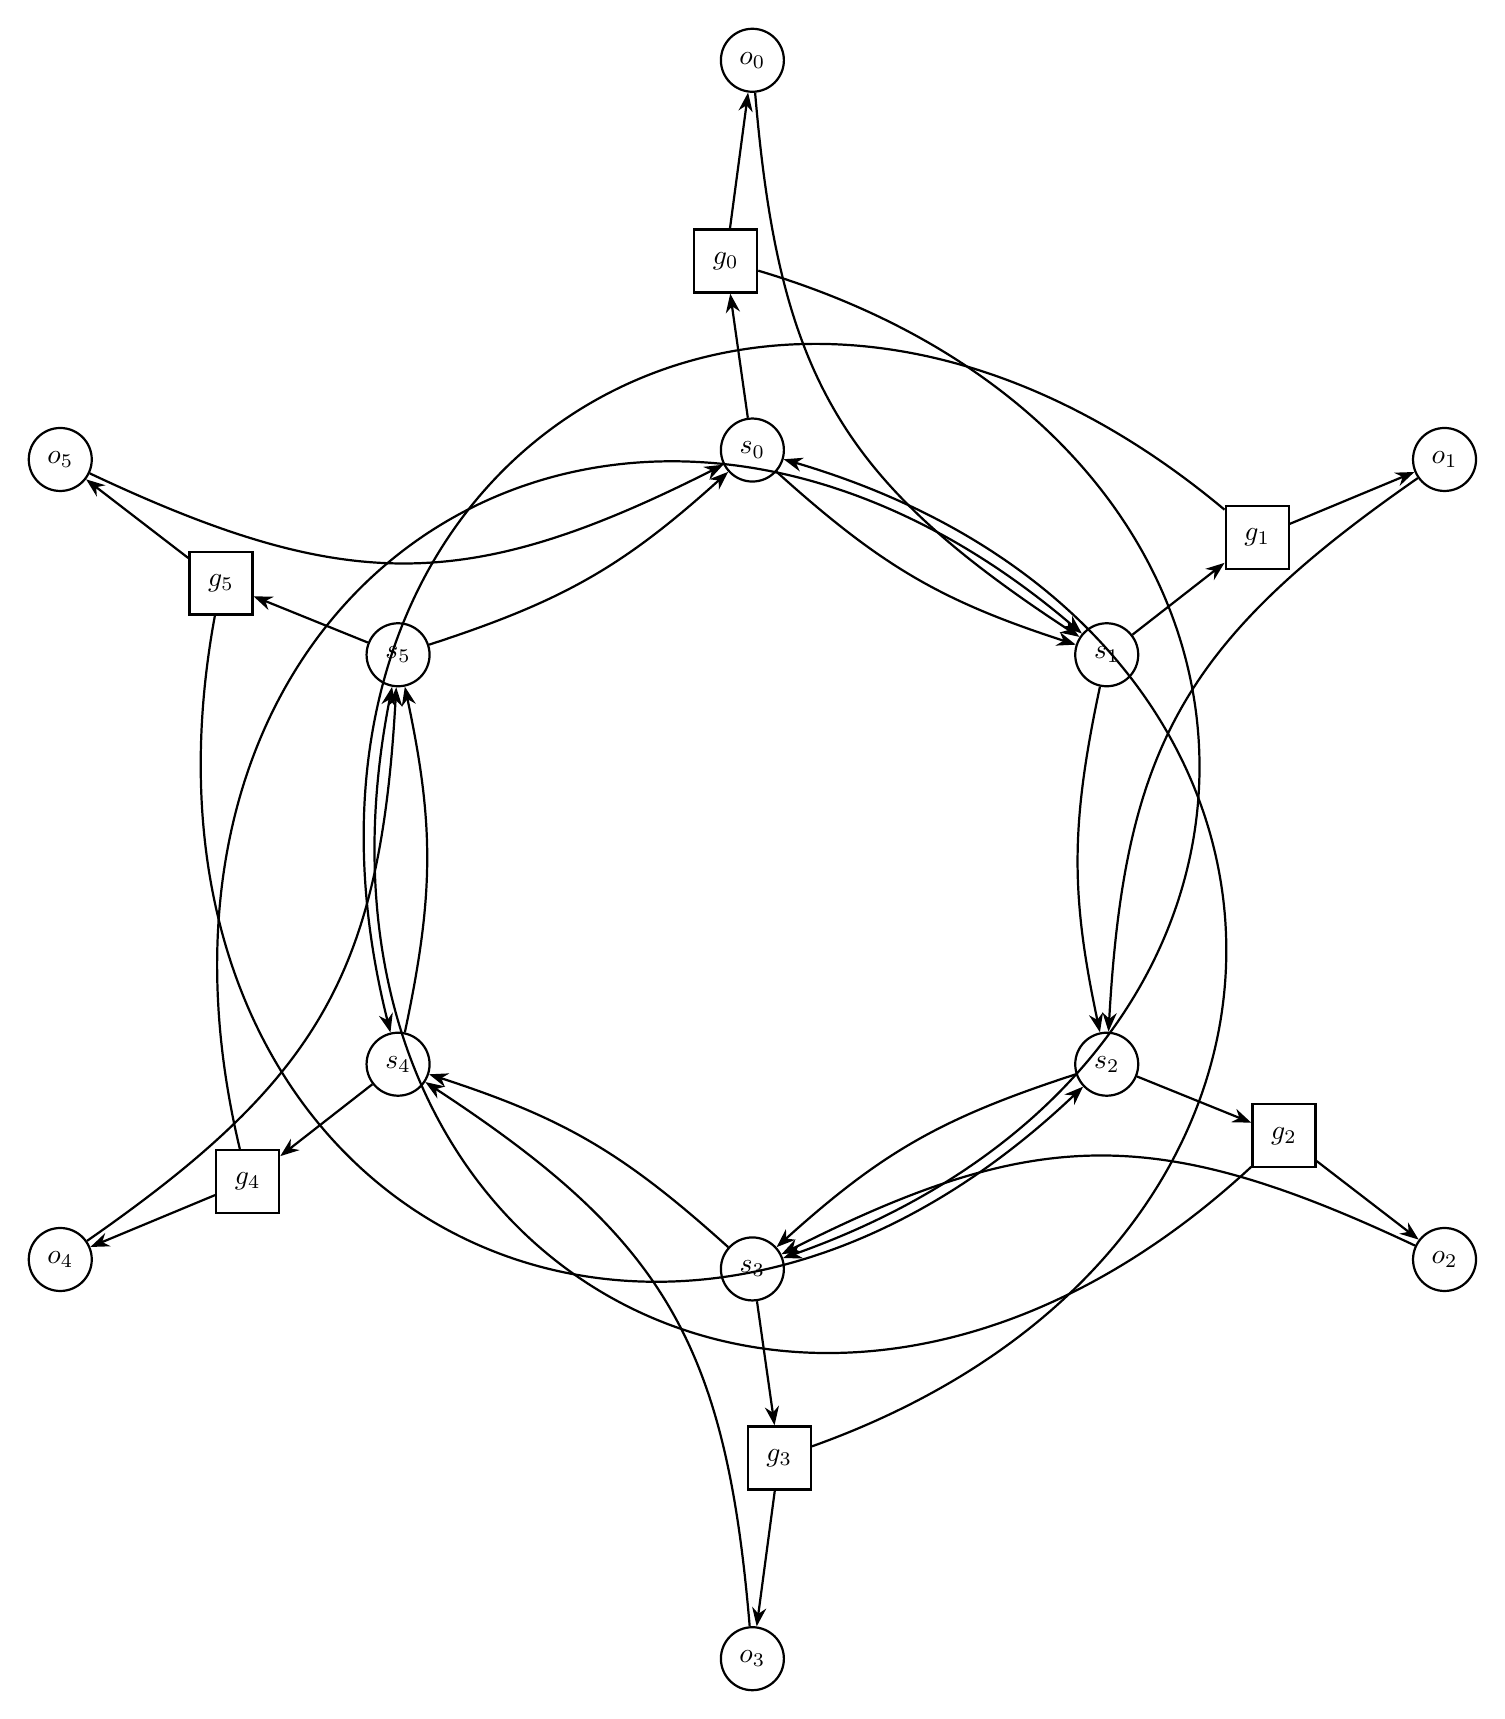
\begin{tikzpicture}[x=1cm,y=1cm]
\tikzset{
  graphnode/.style={circle,draw,thick,minimum size=8mm,inner sep=1pt,font=\sffamily},
  directed/.style={-{Stealth[length=2.4mm]},thick},
  undirected/.style={thick}
}
\node[graphnode,circle,draw] (n_s0) at (0.00,5.20) {$s_{0}$};
\node[graphnode,circle,draw] (n_s1) at (4.50,2.60) {$s_{1}$};
\node[graphnode,circle,draw] (n_s2) at (4.50,-2.60) {$s_{2}$};
\node[graphnode,circle,draw] (n_s3) at (0.00,-5.20) {$s_{3}$};
\node[graphnode,circle,draw] (n_s4) at (-4.50,-2.60) {$s_{4}$};
\node[graphnode,circle,draw] (n_s5) at (-4.50,2.60) {$s_{5}$};
\node[graphnode,rectangle,draw] (n_g0) at (-0.34,7.60) {$g_{0}$};
\node[graphnode,rectangle,draw] (n_g1) at (6.41,4.09) {$g_{1}$};
\node[graphnode,rectangle,draw] (n_g2) at (6.75,-3.51) {$g_{2}$};
\node[graphnode,rectangle,draw] (n_g3) at (0.34,-7.60) {$g_{3}$};
\node[graphnode,rectangle,draw] (n_g4) at (-6.41,-4.09) {$g_{4}$};
\node[graphnode,rectangle,draw] (n_g5) at (-6.75,3.51) {$g_{5}$};
\node[graphnode,circle,draw] (n_o0) at (0.00,10.15) {$o_{0}$};
\node[graphnode,circle,draw] (n_o1) at (8.79,5.08) {$o_{1}$};
\node[graphnode,circle,draw] (n_o2) at (8.79,-5.08) {$o_{2}$};
\node[graphnode,circle,draw] (n_o3) at (0.00,-10.15) {$o_{3}$};
\node[graphnode,circle,draw] (n_o4) at (-8.79,-5.08) {$o_{4}$};
\node[graphnode,circle,draw] (n_o5) at (-8.79,5.08) {$o_{5}$};
\draw[directed] (n_s0) to[bend right=12,looseness=1.05] (n_s1);
\draw[directed] (n_s1) to[bend right=12,looseness=1.05] (n_s2);
\draw[directed] (n_s2) to[bend right=12,looseness=1.05] (n_s3);
\draw[directed] (n_s3) to[bend right=12,looseness=1.05] (n_s4);
\draw[directed] (n_s4) to[bend right=12,looseness=1.05] (n_s5);
\draw[directed] (n_s5) to[bend right=12,looseness=1.05] (n_s0);
\draw[directed] (n_s0) -- (n_g0);
\draw[directed] (n_g0) -- (n_o0);
\draw[directed] (n_o0) to[bend right=26,looseness=1.15] (n_s1);
\draw[directed] (n_s1) -- (n_g1);
\draw[directed] (n_g1) -- (n_o1);
\draw[directed] (n_o1) to[bend right=26,looseness=1.15] (n_s2);
\draw[directed] (n_s2) -- (n_g2);
\draw[directed] (n_g2) -- (n_o2);
\draw[directed] (n_o2) to[bend right=26,looseness=1.15] (n_s3);
\draw[directed] (n_s3) -- (n_g3);
\draw[directed] (n_g3) -- (n_o3);
\draw[directed] (n_o3) to[bend right=26,looseness=1.15] (n_s4);
\draw[directed] (n_s4) -- (n_g4);
\draw[directed] (n_g4) -- (n_o4);
\draw[directed] (n_o4) to[bend right=26,looseness=1.15] (n_s5);
\draw[directed] (n_s5) -- (n_g5);
\draw[directed] (n_g5) -- (n_o5);
\draw[directed] (n_o5) to[bend right=26,looseness=1.15] (n_s0);
\draw[directed] (n_g0) to[bend left=72,looseness=1.55] (n_s3);
\draw[directed] (n_g1) to[bend right=72,looseness=1.55] (n_s4);
\draw[directed] (n_g2) to[bend left=72,looseness=1.55] (n_s5);
\draw[directed] (n_g3) to[bend right=72,looseness=1.55] (n_s0);
\draw[directed] (n_g4) to[bend left=72,looseness=1.55] (n_s1);
\draw[directed] (n_g5) to[bend right=72,looseness=1.55] (n_s2);
\end{tikzpicture}
\end{document}
